\documentclass[11pt]{article}
\usepackage{latexsym}
\usepackage{amsmath}
\usepackage{amssymb}
\usepackage{amsthm}
\usepackage{epsfig}
\usepackage[tight]{subfigure}
\usepackage{amsmath}
\usepackage{array}

\DeclareMathOperator*{\minimize}{min}
\DeclareMathOperator*{\maximize}{max}

\usepackage{algorithm}
 %on linux you may need to run sudo apt-get install texlive-full to install algorithm.sys
\usepackage{algorithmic}

\usepackage{verbatim}

\newcommand{\handout}[5]{
  \noindent
  \begin{center}
  \framebox{
    \vbox{
      \hbox to 5.78in { {#1} \hfill #2 }
      \vspace{4mm}
      \hbox to 5.78in { {\Large \hfill #5  \hfill} }
      \vspace{2mm}
      \hbox to 5.78in { {\em #3 \hfill #4} }
    }
  }
  \end{center}
  \vspace*{4mm}
}

\newcommand{\lecture}[5]{\handout{#1}{#2}{#3}{#4}{#5}}
\newcommand{\collision}[0]{\mathrm{collision}}
\newcommand{\nocollision}[0]{\overline{\collision}}

\newcommand*{\QED}{\hfill\ensuremath{\square}}

\newtheorem{theorem}{Theorem}
\newtheorem{corollary}[theorem]{Corollary}
\newtheorem{lemma}[theorem]{Lemma}
\newtheorem{observation}[theorem]{Observation}
\newtheorem{proposition}[theorem]{Proposition}
\newtheorem{definition}[theorem]{Definition}
\newtheorem{claim}[theorem]{Claim}
\newtheorem{fact}[theorem]{Fact}
\newtheorem{assumption}[theorem]{Assumption}
\newtheorem{note}[theorem]{Note}

% 1-inch margins, from fullpage.sty by H.Partl, Version 2, Dec. 15, 1988.
\topmargin 0pt
\advance \topmargin by -\headheight
\advance \topmargin by -\headsep
\textheight 8.9in
\oddsidemargin 0pt
\evensidemargin \oddsidemargin
\marginparwidth 0.5in
\textwidth 6.5in

\parindent 0in
\parskip 1.5ex
%\renewcommand{\baselinestretch}{1.25}

\begin{document}

\lecture{Statistical Techniques in Robotics (16-831, S22)}{Lecture \#15
  (Wednesday, March 16)}{Lecturer: Kris Kitani}{Scribes: Indraneel Patil, Rachel Zheng}{Value-based Model-based Control}

\section{Review}
In the last lecture, we talked about Markov Decision Processes (MDP). MDP is a discrete-time stochastic control process, which is a typical sequence decision making algorithm. The components of an MDP are defined as:
\begin{itemize}
    \item \textbf{State.} The state defines the current situation of the agent (for eg: it can be the exact position of the Robot in the house, or the alignment of its two legs, or its current posture; it depends on how you address the problem) at some time step. There can be finite or infinite states based on the situation. The example mentioned above is a discrete one, while if we define the state as the amount of oil in a vehicle, it would be continuous.

    \item \textbf{Action.} The choice that the agent makes at the current time step with the environment (for eg: it can move its right or left leg, or raise its arm, or lift an object, turn right or left, etc.). We know the set of actions (decisions) that the agent can perform in advance. In this example, it can be move $\{up, down, left, right\}$. Generally, it can allow us to change the current state or the environment.

    \item \textbf{State-Transition Dynamics.} In the real environment, there exists some uncertainty. So we are not for sure what the outcome of it even if we know the state $s$ and the action $a$. And $p(s^{'} |s, a)$ is probability to describe that, which is a the transition dynamics of the environment, and describes the probability that action $a$ in state $s$ will lead to $s^{'}$,

    \item \textbf{Reward Function.} $r(s^{'} |s, a)$ is the immediate reward received from the environment, which help us model the intention of the agents that they want to achieve. By maximizing its reward, we can get closer to what the agent want. For example, we own the amount money of $x$ and we want to earn the number of money $y$. Therefore, the reward function can be the inversely proportional to the difference from the target money.

    \item \textbf{State prior.} $p_0(s)$ is the initial state probability, which describes the probability of the environment or the agent being initialized to state $s_0$.

    \item \textbf{Policy.} As a probability distribution, a policy is the thought process behind picking an action. In practice, it is a probability distribution assigned to the set of actions. Highly rewarding actions will have a high probability and vice versa. If the agent follow the policy $\pi$, it will perform the $s$ with the probability $\pi (a|s)$ under the condition that the current state is $a$.

    \item \textbf{Discount factor.} The variable $\gamma \in$ [0, 1] is the discount factor. The intuition behind using a discount is that there is no certainty about the future rewards; i.e., as important it is to consider the future rewards to increase the Return, it is also equally important to limit the contribution of the future rewards to the Return (Since you can’t be 100\% sure of the future). When we look at an agents behavior over a series of time steps, we generally like to sum all of the rewards at every time step to get the return of the trajectory. In this sum, we can choose to multiply future rewards by a power of $\gamma$ to control the value of weights that we put in the future rewards.
\end{itemize}

\subsection{Pacman world example of an MDP}

\begin{figure}[H]
  \centering
  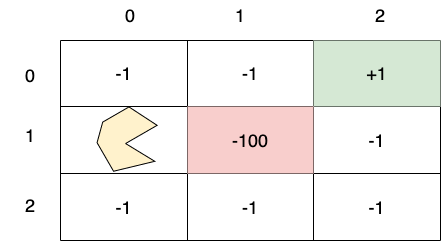
\includegraphics[width=0.75\linewidth]{pacman_new.png}
\caption{Pacman World}
\label{fig:test}
\end{figure}

\subsubsection{Description of the world}
\begin{enumerate}
\item The State : current position of the pacman. As we can see initial state is $(1,0)$ 
\item Actions : Pacman can move either up,down, left or right 
\item Rewards : are drawn on the world itself, apart from the red ghost state and the green cherry state, all other transitions get a reward of -1 
\item Deterministic transitions : Each action from any state has a deterministic end state, in simple words all actions are always considered to be successful
\item What happens when you go off the grid? If at any state you take an action to go off the grid, you are automatically returned to the same state
\item Assume discount factor $ \gamma$ of 0.5 to prefer immediate rewards compared to future rewards
\item Terminating state : In this example ${2,0}$ is the only terminating state
\end{enumerate}


\subsubsection{State value function of (1,0) with policy go right}
$$ V^\pi(s) = E_p[\gamma^0r_0 + \gamma^1r_1 + \gamma^2r_2 ... | s_0 = s]$$
$$ V^{right}(s) = E_p[\gamma^0r_0 + \gamma^1r_1 + \gamma^2r_2 ... | (1,0) = s]$$
$$ V^{right}(1,0) = -100 + 0.5^1*-1 + 0.5^2*-1 ... $$
$ V^{right}(1,0) $ is some large negative number

\subsubsection{State value function of (0,1) with policy go right}
$$ V^\pi(s) = E_p[\gamma^0r_0 + \gamma^1r_1 + \gamma^2r_2 ... | s_0 = s]$$
$$ V^{right}(s) = E_p[\gamma^0r_0 + \gamma^1r_1 + \gamma^2r_2 ... | (0,1) = s]$$
$$ V^{right}(0,1) = +1 $$
$ V^{right}(0,1) $ is +1 because we reached the terminating state in one step

\subsubsection{State value function of (0,0) with policy go right}
$$ V^\pi(s) = E_p[\gamma^0r_0 + \gamma^1r_1 + \gamma^2r_2 ... | s_0 = s]$$
$$ V^{right}(s) = E_p[\gamma^0r_0 + \gamma^1r_1 + \gamma^2r_2 ... | (0,0) = s]$$
$$ V^{right}(0,0) = -1 +1*0.5^1 $$
$$ V^{right}(0,0) = -0.5 $$
$ V^{right}(0,0) $ is +0.5 because we reached the terminating state in two steps

\subsubsection{State-action value function of (1,0) with action up policy go right}
$$ Q^\pi(s,a) = E_p[\gamma^0r(s_0) + \gamma^1r(s_1) + \gamma^2r(s_2) ... | s_0 = s, a_0 = a]$$
$$ Q^{right}((1,0),up) = E_p[\gamma^0r(1,0) + \gamma^1r(s_1) + \gamma^2r(s_2) ... | (1,0) = s, up = a]$$
$$ Q^{right}((1,0),up) = -1 + 0.5^1*-1 +0.5^2*1$$
$$ Q^{right}((1,0),up) = -1.25$$

\subsection{Bellman equation intuition}
Bellman equation as we will see from its mathematical formulation is a way of representing the value of a state in the MDP (future expected reward) in terms of the value of its adjacent states. This gives us a handy way of evaluating the values of all states in the MDP in a recursive way.
$$ V^\pi(s) = \sum_a \pi(a|s)^{(1)} \sum_{s`} p(s`|s,a)^{(2)}[r(s`,a,s)^{(3)} + \gamma V^\pi(s`)^{(4)}] $$
\begin{enumerate}
    \item Sum over all possible actions that can be taken under policy $\pi$ from this state
    \item Sum over all possible states that can result from taking this action multiplied by its transition probability
    \item Reward of that particular transition
    \item Discounted future expected reward from the resulting state by following policy $\pi$ until the end of time
\end{enumerate}

\subsection{Bellman optimality equation intuition}
Bellman optimality equation gives us the maximum expected future reward from any given state because we are following the optimal policy in the MDP. Unlike the bellman equation, we dont consider all possible actions from the state but only the best one which leads to the best reward, so the summation is replaced by maximisation.
$$ V^{\pi^*}(s) = \max_a^{(1)} \sum_{s`} p(s`|s,a)^{(2)}[r_t^{(3)} + \gamma V^{\pi^*}(s`)^{(4)}] $$
\begin{enumerate}
    \item Select the best possible action from this state
    \item Sum over all possible states that can result from taking this action multiplied by its transition probability
    \item Reward of that particular transition
    \item Discounted future expected reward from the resulting state by following the best possible policy $\pi$ until the end of time
\end{enumerate}

%This section serves as a review of the previous lecture and any other context required to frame the content of the current lecture. 

%You may format the scribes in any way you like, aside from changing font style, size and page format. Please use subsections and paragraphs to increase the readability of your notes.

%Length requirement 1-2 pages.
        

\section{Model Based control}

\subsection{Problem setup}
We can model an MDP with a closed loop control system using policy and value iteration. The control system loops between policy evaluation and improvement stages.

\begin{figure}[H]
    \centering
    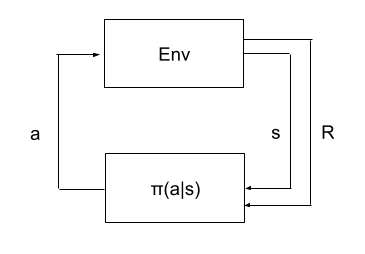
\includegraphics[width=0.4\linewidth]{model based.png}
    \caption{MDP as Control Problem}
    \label{fig:my_label}
\end{figure}

\subsection{Policy Iteration}
Policy iteration is a way of finding an optimal policy. Once a policy, $\pi$, has been improved using $V^{\pi}$ to yield a better policy, $\pi'$, we can then compute $V^{\pi'}$ and improve it again to yield an even better policy. We can thus obtain a sequence of monotonically improving policies and value functions.\\
Each policy is guaranteed to be a strict improvement over the previous one (unless it is already optimal). Because a finite MDP has only a finite number of policies, this process must converge to an optimal policy and optimal value function in a finite number of iterations.

\begin{figure}[H]
    \centering
    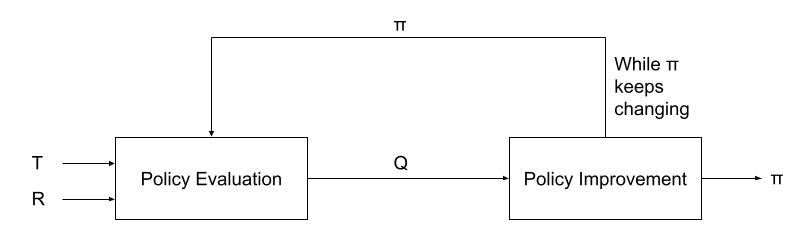
\includegraphics[width=0.8\linewidth]{Policy iteration.png}
    \caption{Policy Iteration}
    \label{fig:my_label}
\end{figure}

In policy iteration, the agent evaluates $V$ given a our current $\pi$, and then improves it using $V$, which causes $V$ to change and so on. The loop continues until $\pi$ stays the same after improvement.\\
Policy evaluation takes an existing $\pi$ and computes $Q$ for that current policy.
Then, the agent uses $Q$ to improve the policy.\\
Policy iteration has converged once the policy does not change after improvement.

\begin{algorithm}
\caption{Policy Evaluation}\label{alg:cap}
\begin{algorithmic}[1]
\STATE $V \gets rand(\mathbb{R})$
\STATE $V' \gets rand(\mathbb{R})$
\WHILE{$\max_s |V(s)-V'(s)|\geq \epsilon$}
    \STATE $V' \gets V$
    \FOR{$s \in S$}
        \STATE $Q(s,a) = r(s) + \gamma \sum\limits_{s'} p(s'|s,a)V'(s') \quad \forall a$
        \STATE $V(s) = \sum\limits_a \pi(a|s)Q(s,a)$
    \ENDFOR
\ENDWHILE
\RETURN $Q$
\end{algorithmic}
\end{algorithm}

\begin{algorithm}
\caption{Policy Iteration}
\label{algo:policy}
\begin{algorithmic}[1]
\STATE $\pi \gets rand(\mathcal{A})$
\WHILE{$\pi$ is changing}

\STATE $Q(s,a) \gets \text{PolicyEvaluation}(\pi, r(s), p(s'|s,a), \gamma)$
\FOR{$s\in\mathcal{S}$}
    \STATE $\pi(s) = \text{argmax}_a Q(s,a)$
\ENDFOR
\ENDWHILE
\end{algorithmic}
\end{algorithm}

\subsection{Why does Policy iteration produce the optimal policy?}
We know that the best policy should get the greatest expected return for all states: \\
$$ V^{\pi^*}(s) = \max_\pi V^\pi(s)$$ 
$$ Q^{\pi^*}(s,a) = \max_\pi Q^\pi(s,a)$$ 

We can prove that policy iteration produces monotonic improvement in the value function for each iteration. We initialise our policy randomly $\pi \gets rand(\mathcal{A})$, Lets call this policy $\pi_1$. then we evaluate this policy using the bellman equation for all states and actions.
$$Q^{\pi_1}(s,a) = r(s) + \gamma \sum\limits_{s'} p(s'|s,a)V^{\pi_1}(s') $$
$$ V^{\pi_1}(s) = \sum_a \pi(a|s)Q(s,a)  $$

In the policy iteration step, we calculate a policy which maximises the expected return for all states based on our current value function. So we select a policy $\pi_2$ which strictly improves $V^{\pi_1}(s)$
$$ \pi_2(s) = \text{argmax}_a Q^{\pi_1}(s,a)$$
$$ Q^{\pi_1}(s,\pi_2) \geq V^{\pi_1}(s)  $$

Substituting this result in the above equation for $V^{\pi_1}(s) $ we get,
$$ V^{\pi_1}(s) \leq  r(s) + \gamma \sum\limits_{s'} p(s'|s,\pi_2)Q^{\pi_1}(s',\pi_2) $$
$$ V^{\pi_1}(s) \leq  r(s) + \gamma*r(s) + \gamma^2 \sum\limits_{s'} p(s'|s,\pi_2)V^{\pi_2}(s') $$
$$ V^{\pi_1}(s) \leq V^{\pi_2}(s) $$

Convergence condition for policy iteration is,
$$ V^{\pi_k}(s) = V^{\pi_{k+1}}(s) $$

For this to hold true, $V^{\pi_k}(s) $ must also satisfy the bellman optimality condition
$$ V^{\pi^k}(s) = \max_a \sum_{s`} p(s`|s,a)[r_t + \gamma V^{\pi^k}(s`)] $$

Hence at convergence of policy iteration we get $ V^{\pi_k}(s) = V^{\pi_*}(s) $ which is the optimal policy we wanted.



\subsection{Value Iteration}
In value iteration, the policy is improved in the same loop as the value function.
Value iteration is simpler and takes direct advantage of dynamic programming.
\begin{figure}[H]
    \centering
    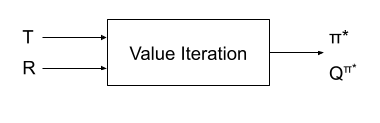
\includegraphics[width=0.4\linewidth]{Value iteration.png}
    \caption{Value Iteration}
    \label{fig:my_label}
\end{figure}

The value iteration algorithm initializes with a random policy. At the evaluation step, for each state, it uses the Bellman Optimality Equation to calculate the state-action value for every action. It then selects the state-action pair with the maximum value as the optimal policy. The improvement takes the optimal policy and uses it to update the optimal values. THe algorithm repeats until the values for each state no longer change. The final value is then the optimal value.

\begin{algorithm}
\caption{Value Iteration}\label{alg:cap}
\begin{algorithmic}[1]
\STATE $\pi \gets rand(\mathcal{A})$
\STATE $V \gets rand(\mathbb{R})$
\STATE $V' \gets rand(\mathbb{R})$
\WHILE{$\max_s |V(s)-V'(s)|\geq \epsilon$}
    \STATE $V' \gets V$
    \FOR{$s \in S$}
        \STATE $Q(s,a) = r(s) + \gamma \sum\limits_{s'} p(s'|s,a)V'(s') \quad \forall a$
        \STATE $\pi(s) = \text{argmax}_a Q(s,a)$
        \STATE $V(s) = Q(s,\pi(s))$
    \ENDFOR
\ENDWHILE\\
\end{algorithmic}
\end{algorithm}



\subsection{Which converges faster? Policy or Value?}
One drawback to policy iteration is that each of its iterations involves policy evaluation, which may itself be a protracted iterative computation requiring multiple sweeps through the state set. If policy evaluation is done iteratively, then convergence exactly to  occurs only in the limit. Must we wait for exact convergence, or can we stop short of that?\\
In fact, the policy evaluation step of policy iteration can be truncated in several ways without losing the convergence guarantees of policy iteration. When policy evaluation is stopped after just one sweep, it becomes Value Iteration.\\
Value iteration effectively combines, in each of its sweeps, one sweep of policy evaluation and one sweep of policy improvement. Faster convergence is often achieved by interposing multiple policy evaluation sweeps between each policy improvement sweep. \\

\textbf{Practical application} \\

In practice however if our initial policy is very wrong, value iteration can take a long time to converge so often value iteration and policy iteration are used one after the other to overcome the drawbacks of one another.


\section{Reinforcement Learning}
Reinforcement Learning maps situations
to actions to maximize a reward signal. In problems of complete knowledge, the agent has a complete and accurate model of the environment's dynamics. If the environment is an MDP, then such a model consists of the one-step transition probabilities and expected rewards for all states and their allowable actions. In our formulation, we used a model of the state transition dynamic and reward function. This is called Model-Based RL.\\
In problems of incomplete knowledge, a complete and perfect model of the environment is not available. This is called Model-Free RL. Model-Free RL can be thought of as an "explicit" trial-and-error algorithm.

\subsection{Difference between RL and Optimal control}
\begin{center}
\begin{tabular}{ | m{3cm} | m{6cm}| m{6cm} | } 
  \hline
  _ & \textbf{Reinforcement learning} & \textbf{Optimal control} \\ 
  \hline
  \textbf{Definition} & mapping situations to actions to maximise a reward signal & find a sequence of actions that when executed, result in state-action pairs with low cumulative cost \\ 
  \hline
  \textbf{Objective} & Maximise reward & Minimise cost \\ 
  \hline
  \textbf{Modeling environment} & Common methods include using tables or neural networks  & Usually an underlying physics dynamical model is used \\ 
  \hline
  \textbf{System lingo} & Environment  & Plant \\ 
  \hline
  \textbf{Decision maker lingo} & Agent/Policy  & Controller \\ 
  \hline
\end{tabular}
\end{center}

Apart from the above noted semantics, both techniques have the same end goal which is \textbf{to produce some desirable behaviour from the system subject to certain constraints}.


\subsection{Difference between RL and Bandit setting}
\begin{enumerate}
\item Both RL and multi armed bandit problems have evaluative feedback so the loss is occluded.
\item They both can have sampled feedback, so you dont get to see all the possible situations
\item The main difference is that bandits are a one shot feedback problems, so outcome of one action does not affect the next trial whereas RL is a sequential feedback problem, so one action affects the next trial in the sequence.
\end{enumerate}


\section{Challenges in Model Based control}
\begin{enumerate}
\item Real world is often only partially observable, so for example for a car the pedastrians crossing the road maybe occluded by another car we are trying to overtake
\item Real world dynamics are often hard to model and hence it is difficult to simulate state transitions on new actions taken by the policy
\item All the system constraints must be baked into the reward functions so that system produces desirable behaviour on maximising this reward function, but designing reward functions is not always straightforward.
\end{enumerate}




%\section*{References}
%Include your references here. Please cite any resources you found useful.	
%Populate the refs.bib file or list your references manually. Be consistent in formatting!
{
\bibliography{refs}
\bibliographystyle{abbrv}
}

%\section{Appendix}
%This section provides any relevant background material that was not covered in the lectures, but was found to be useful for understanding the material. 
%For example, derivations, theory underlying techniques employed, etc. 

%Additionally, this section can summarizes applications or extensions of these techniques found in the literature. 

\end{document} % Done!


